\chapter{Evaluation}\label{C:eval}

\section{Accuracy Testing}

The aim for the following tests is to assess how accurate the device is. For a device to be useful, it needs to be 
able to measure latency with both accuracy and precision. Precision is the difference between repeated tests and 
this is limited by the clock cycles provided to the timing module. Accuracy is how close the measured value is to 
the theoretical value and dependant on the filtering and post processing done with the data received by the timing 
module. 

The results are expected to be the same over different tests, as the same cable will be used for each packet sent. 
The latency should increase linearly with the length of the cable, as the speed of light and velocity factor is 
constant.

\begin{figure}[H]
    \begin{center}
        
\includegraphics[keepaspectratio,height=8.5cm]{Images/TestSetup}
        \caption{Measurement setup for 4 different tests (4 cm, 3 m, 25 m and 2 m)}
        \label{fig:testSetup}
    \end{center}
\end{figure}

To test the accuracy of the device, a loopback test was performed with different length of cables. This was setup so 
that there was no switch between two ethernet measurement ports, only an ethernet cable. The test is to ensure that 
the device is measuring the latency correctly, and able to detect the latency present in a specific length of cable. 
Latency measured from the device can be compared with the theoretical value of the latency which can be calculated 
using the following formula:

\[ Latency = \frac{L}{cV_f} \] 

Where L is the length of the cable, c is the speed of light (299,792,458 m/s) and V\textsubscript{f} is velocity 
factor of ethernet cables (0.65 (REFERENCE HERE)).

A very short cable (4 cm) was used to measure the processing time, a constant added to every measurement. This 
processing time is the result of both Ethernet Phys converting between the two protocols (Differential Pairs and 
RGMII). A short cable produces an immeasurable latency which is beyond the precision of the device, deducing that 
the latency measured from this test would be because of the constant processing on board the device. Performing 
measurements with the short cable produced a mean value of 440 ns where 0.2095 ns of the measurement is attributed 
to the delay present in the cable (5\% of the precision of the device). 

This processing time is then removed from subsequent tests, making the latency values produced by the device purely 
the latency present in the cable. The goal from the tests is to ensure that the device is accurate to within 4 ns, 
which is the smallest interval of time that can be measured. 

Tests were done with cables spanning 2 m, 3 m and 25 m long. These provided enough of a delay to measure with the 
device and enough data to characterise latency present in the cables. The measured value was plotted with the 
theoretical values of what delay would be present in the cable. To obtain the delay measurement, the test was run 
for 20 seconds on the device, with a packet transmission frequency of 500 packets per second. The mean value of all 
packet latency measurements for that cable were then plotted versus the length of the cable.

\begin{figure}[H]
    \begin{center}
        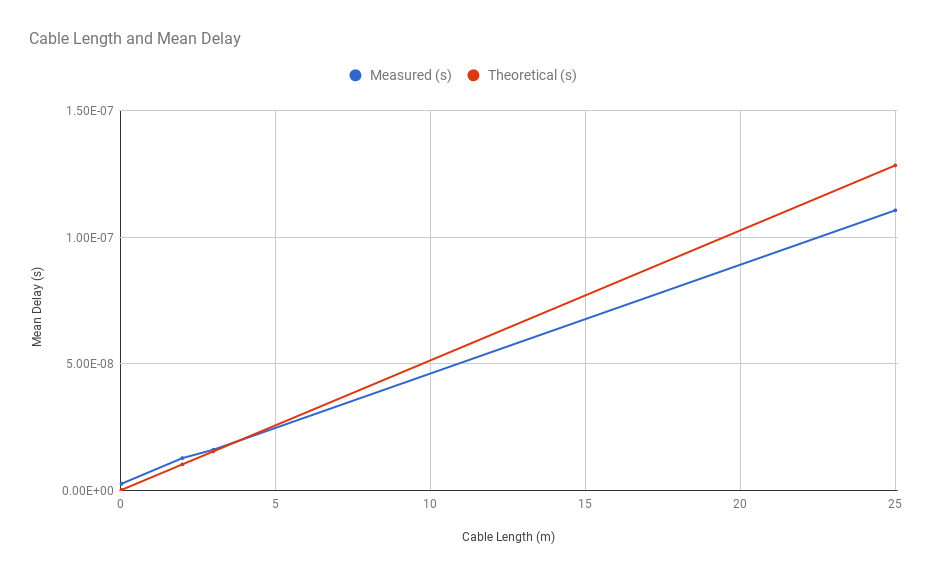
\includegraphics[keepaspectratio,height=7.5cm]{Images/CableTesting}
        \caption{Results from FPGA device latency accuracy measurements with 0.65 Velocity Factor}
        \label{fig:cableTesting}
    \end{center}
\end{figure}

As shown in Figure \ref{fig:cableTesting}, the results from the device show a linear trend in latency due to length 
of the cable. The velocity factor was obtained from (CITE HERE) and a change in velocity factor could be a factor 
for the discrepancies found in the gradients. The values have an error of ±4 ns as the points fluctuated above and 
below a certain value and the average was plotted. There were no outliers during testing, showing how the device is 
not prone to producing wildly different results.

\begin{figure}[H]
    \begin{center}
        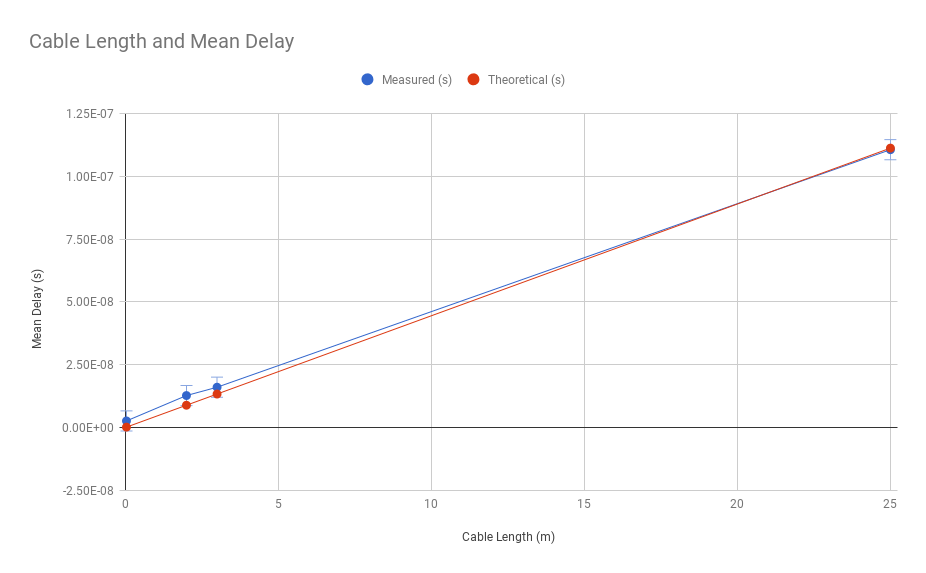
\includegraphics[keepaspectratio,height=7.5cm]{Images/CableTesting075}
        \caption{Results from FPGA device latency accuracy measurements with 0.75 Velocity Factor}
        \label{fig:cableTesting075}
    \end{center}
\end{figure}

An interesting point in Figure \ref{fig:cableTesting} is that the 25 m measurement was less than the theoretical 
value. The velocity factor appears to be the main cause of this difference, as the speed of light cannot change and 
different cables tend to have different velocity factors and this is shown in Figure \ref{fig:cableTesting075}. With 
the velocity factor altered to 0.75, this makes device appear more accurate. The standard deviation of the 25 m test 
is 2.4 ns, with a range of 8 ns.

From the results given, it is accurate to within 4 ns when measuring short ranged cables of 2-3 m and the longer the 
cables become, the worse the measurement becomes. This could be caused by discrepancies in the velocity factor of 
ethernet cables.

\section{Reliability Testing}

Reliability is a key project goal of this device and to test this, a real-world scenario was replicated. As the 
project is to create a device which can measure reliably, the following tests would be how similar independent tests 
measure the latency. If repeated tests are done on a reliable device, they should be around the same measurement 
value.

To test reliability of the device, repeated tests were performed to understand how consistent the values are from 
test to test. As the goal of the project was to measure the latency in network switches, these tests were to measure 
the latency through a network switch and provide repeatable results. The results do not need to be accurate, as the 
accuracy was determined in the test in accuracy testing, hence these results are only to measure the reliability. 

Results from the tests were compared to an existing PF\textunderscore RING software based latency measurement method.
This was run on two separate machines which had clocks synchronised using PTP protocol and as a result, the timings 
varied significantly. This comparison was to show that the software based methods have flexibility that hardware 
methods are missing while also performing unreliably. 

The PF\textunderscore RING based system was compared to the FPGA based device by producing a packet on one machine, 
then sending the packet through the network switch to arrive at the other machine, and the time delta is returned 
from both machines. The FPGA device also performed the same task with the same cables, but the two connections 
arrived at the same machine. This test is assumed to take a constant time which would not change over independent 
tests as the network switch would be not switching extra traffic and the MAC learning table inside the device would 
have learned the route for the network packets by the first network packet. 

\begin{figure}[H]
    \begin{center}
        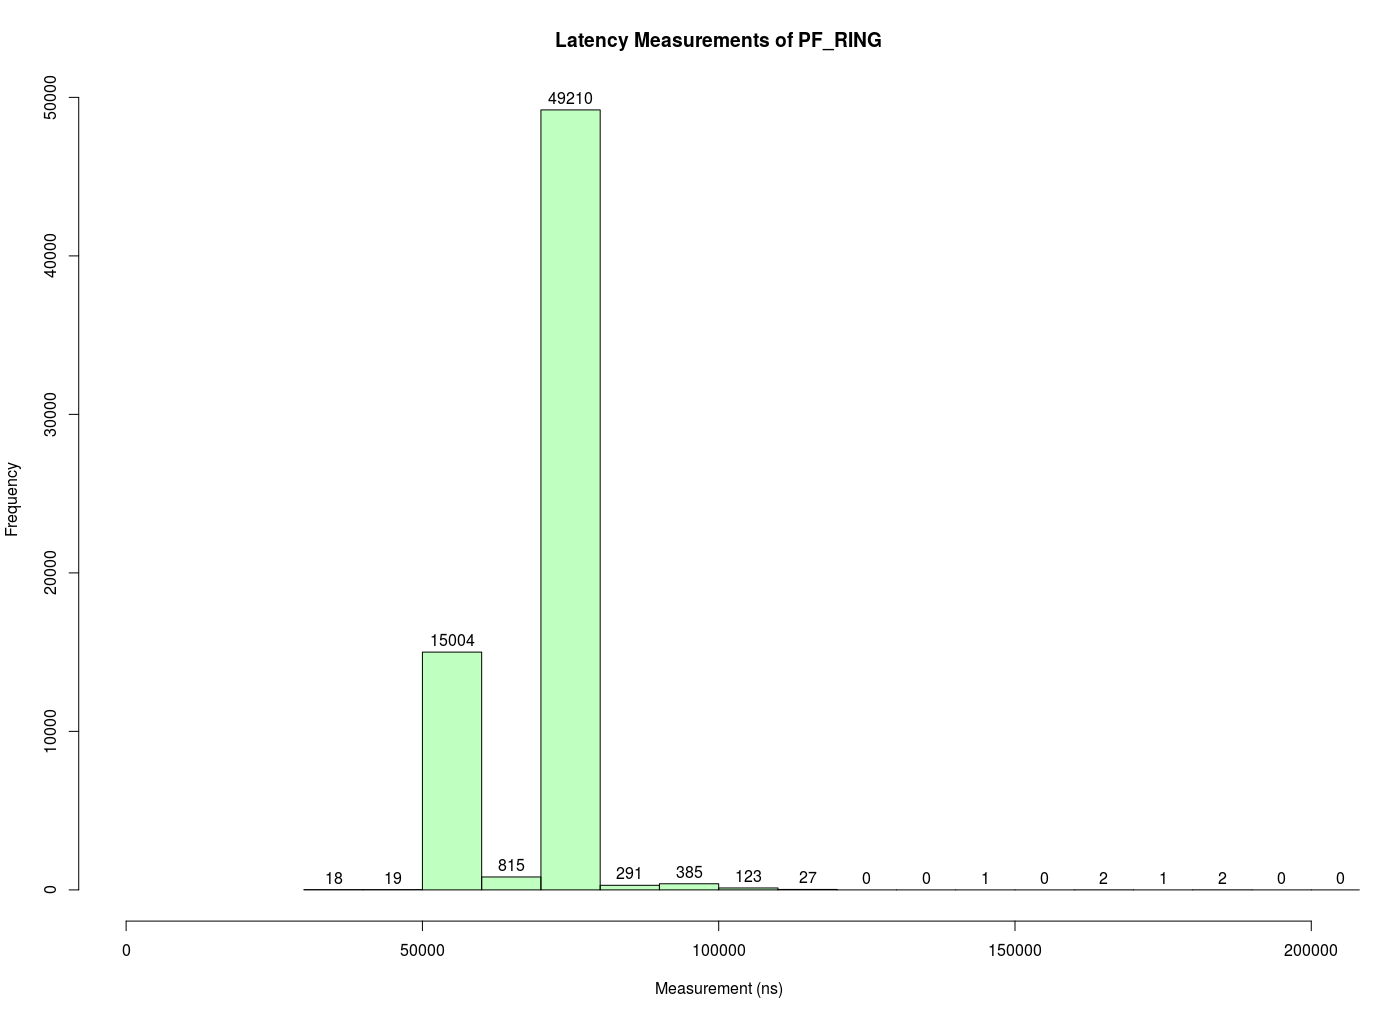
\includegraphics[keepaspectratio,height=7.5cm]{Images/pf_ring}
        \caption{Results from DPDK Reliability Measurements}
        \label{fig:DPDKReliability}
    \end{center}
\end{figure}

Results from running PF\textunderscore RING latency measurements shows the spread in measurements due to 
inconsistencies in the delay from getting a measurement value. As this is a software based platform, there are many 
queues and buffers inside both the operating system and the hardware interfaces. This inconsitency more detailed in 
the introduction to the report.

\begin{figure}[H]
    \begin{center}
        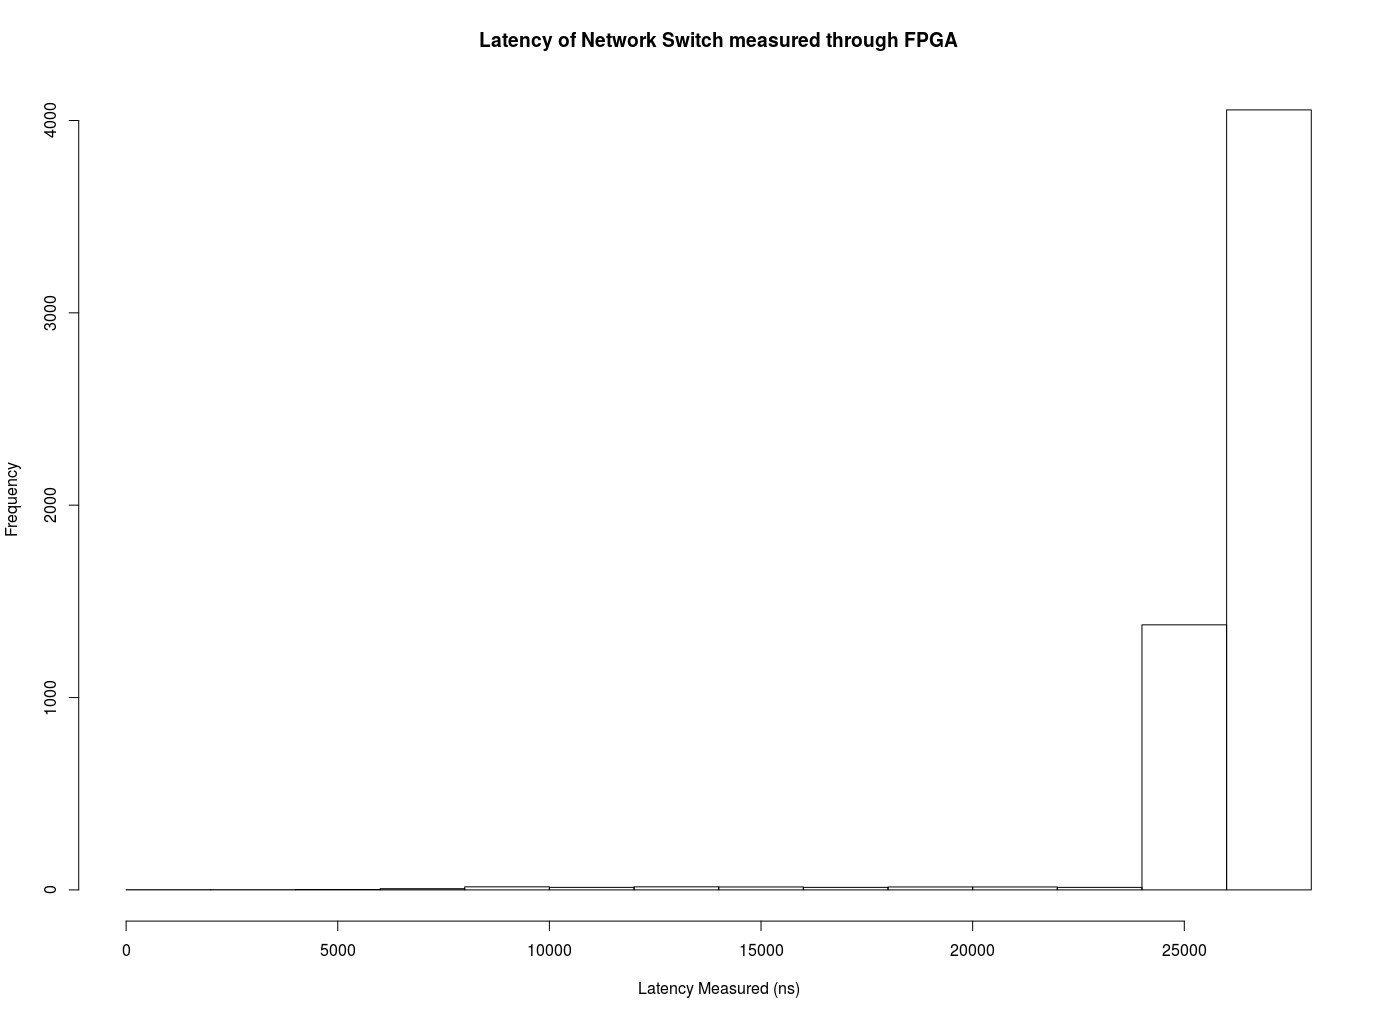
\includegraphics[keepaspectratio,height=7.5cm]{Images/TestPlot}
        \caption{Results from FPGA device Reliability Measurements}
        \label{fig:Test2Plot}
    \end{center}
\end{figure}

Data from the FPGA device showed that the measurements were only under estimated, and the device never overestimated.
This is interesting as the device also had some measurements where the latency was 0 ns through the switch, which is 
impossible to achieve. The spread over all the measurements was quite lower than the PF\textunderscore RING 
statistics, and overall the mean was 36\% of the PF\textunderscore RING measurement mean. 

\begin{figure}[H]
    \begin{center}
        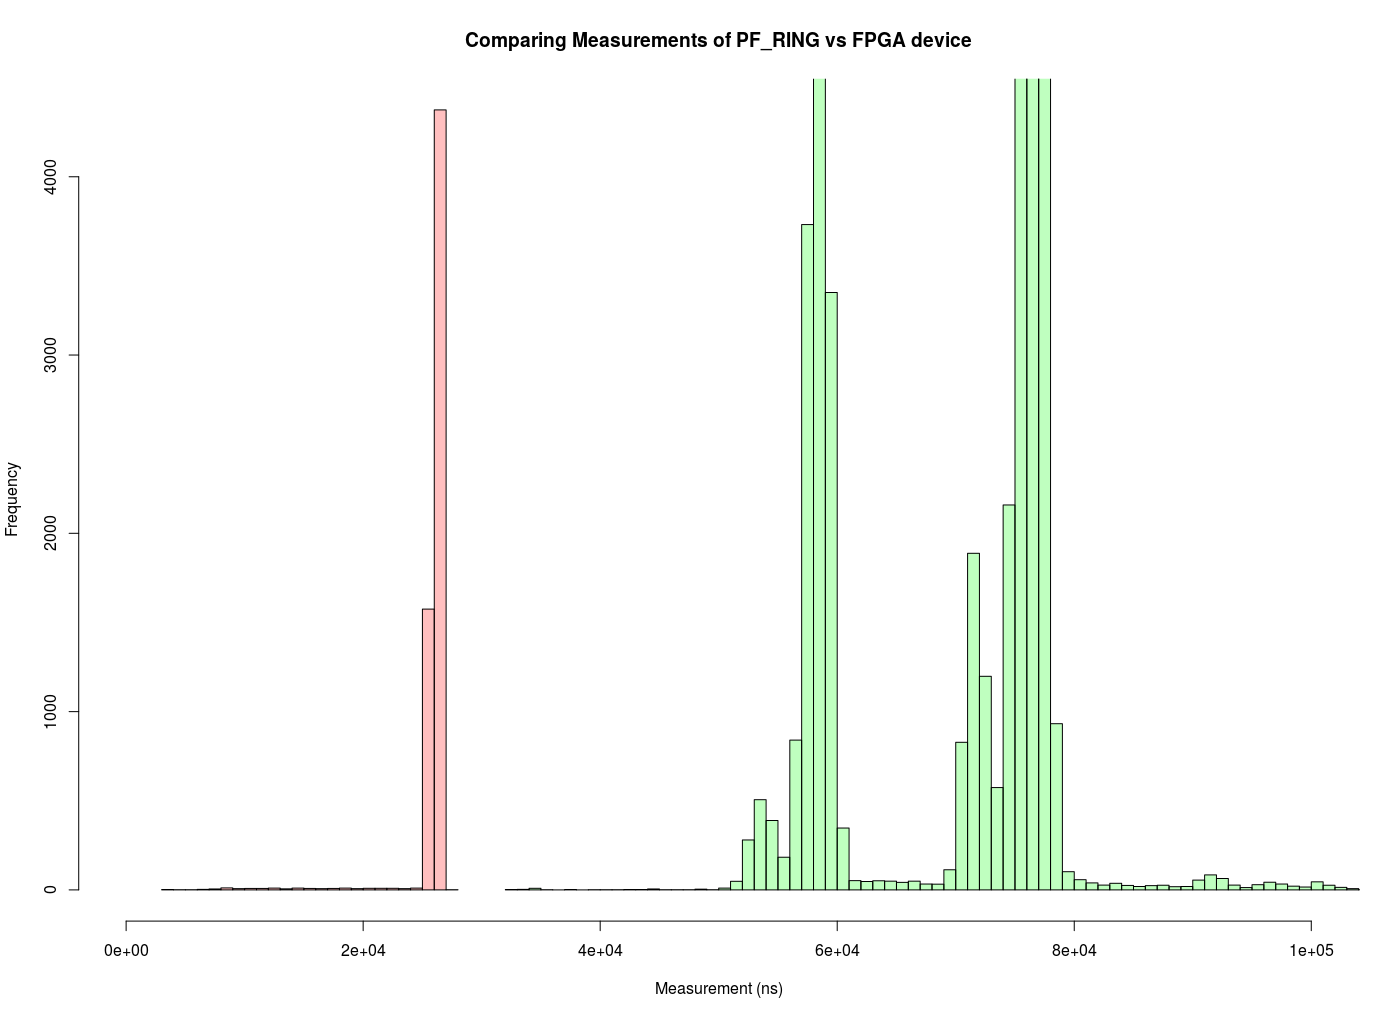
\includegraphics[keepaspectratio,height=7.5cm]{Images/Comparision}
        \caption{Comparision of the results from PF\textunderscore RING and the FPGA device}
        \label{fig:comparision}
    \end{center}
\end{figure}

Figure \ref{fig:comparision} shows the difference between the two testing methods. As seen, the PF\textunderscore 
RING measurements show 2.8x increase in mean latency, most likely produced by the overhead of using an operating 
system and CPU stack. These tests are only meant to measure the difference in spread of the measurement, so to 
counter the discrepancies in the means, Coefficient of Variation is used to remove the varying factor of the mean 
causing a change in standard deviation.

\begin{table}[h!]
    \begin{center}
        \begin{tabular}{ |p{9cm}||p{2.5cm}|p{2.5cm}| }
            \hline
            Device & FPGA Device & PF\textunderscore RING\\
            \hline
            Standard Deviation & 1878.23 & 20754.18\\
            Mean & 25989.76 & 72431.35\\
            Coefficient of Variation & 0.07 & 0.28\\
            Standard Deviation Improvement vs PF\textunderscore RING & 11.04 & 1\\
            Coefficient of Variation Improvement vs PF\textunderscore RING & 3.96 & 1\\
            \hline
        \end{tabular}
        \caption{Statistics of results}
        \label{table:stats}
    \end{center}
\end{table}

Comparing the two from a statistical point of view, it can be concluded that the FPGA device is more capable of 
producing a more reliable measurement. The standard deviation of the FPGA device is over 11x of a reduction over the 
software based PF\textunderscore RING. The discrepancy in the means is something to note, but not part of this test. 
The accuracy of PF\textunderscore RING could be future test, to understand if the device is as accurate as the FPGA 
device, but the aim for these tests was to compare the repeatability of latency measurements. 
